\documentclass[11pt]{article}
\usepackage[margin=1in]{geometry}
\usepackage{amsmath,amssymb}
\usepackage{booktabs}
\usepackage{xcolor}
\usepackage{tikz}
\usetikzlibrary{positioning,arrows.meta,fit,backgrounds,calc,shapes.geometric}
\usepackage[colorlinks=true,linkcolor=blue,urlcolor=blue]{hyperref}

\definecolor{cset}{RGB}{31,119,180}
\definecolor{cfield}{RGB}{44,160,44}
\definecolor{cop}{RGB}{214,39,40}
\definecolor{cgray}{RGB}{120,120,120}

\title{\textbf{TissueGraph}\\[2pt]
\large Hierarchical sets and operators for differentiable tissue}
\author{Janelia Research Campus}
\date{\today}

\begin{document}
\maketitle

\begin{abstract}
Living tissues couple biochemical signalling, cellular interaction, mechanical
force, and collective dynamics across scales. The frameworks built so far
(\textsc{CellGraph}, \textsc{NeuralGraph}, \textsc{MPMGraph},
\textsc{MetabolismGraph}) each implement \emph{one} graph type. A tissue needs
them coexisting. We define the missing primitive: a \textbf{hierarchical graph
container} stated in the language of \textbf{sets} and \textbf{operators}. A
tissue is a stack of sets linked by containment; dynamics are operators --- GNNs
implementing ODE vector fields and Laplacians --- dispatched by relation. Every
existing framework becomes a set of registered operators plus a schedule.
\end{abstract}

\section{Two entities: sets and fields}

A \textbf{set} $S_k$ is a collection of like nodes at scale $k$ (molecules,
particles, cells, populations). The hierarchy is a sequence of \textbf{partitions}
\[
\pi_k : S_k \longrightarrow S_{k+1},
\]
so that a cell \emph{is} the fibre $\pi_1^{-1}(c)$ of its particles. A
\textbf{field} $f:\Omega\to\mathbb{R}^c$ is a continuum on its own grid, bound to
one level. Fields do not nest; they form a flat set, each tagged with the level
it couples to (Fig.~\ref{fig:hier}).

\begin{figure}[h]
\centering
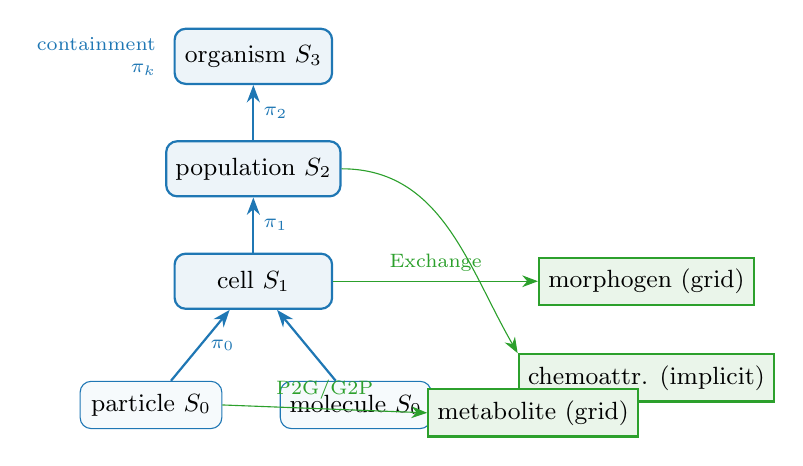
\begin{tikzpicture}[
  font=\small,
  set/.style={draw=cset,thick,rounded corners,fill=cset!8,minimum width=20mm,minimum height=7mm},
  leaf/.style={draw=cset,fill=cset!4,rounded corners,minimum width=18mm,minimum height=6mm},
  fld/.style={draw=cfield,thick,fill=cfield!10,minimum width=22mm,minimum height=6mm},
  rel/.style={-{Stealth[length=2mm]},cgray},
  cont/.style={-{Stealth[length=2.2mm]},cset,thick},
]
% hierarchy spine
\node[set] (org) {organism $S_3$};
\node[set,below=7mm of org] (pop) {population $S_2$};
\node[set,below=7mm of pop] (cell) {cell $S_1$};
\node[leaf,below=9mm of cell,xshift=-13mm] (part) {particle $S_0$};
\node[leaf,below=9mm of cell,xshift=13mm] (mol) {molecule $S_0$};

\draw[cont] (part) -- node[right,font=\scriptsize,cset]{$\pi_0$} (cell);
\draw[cont] (mol) -- (cell);
\draw[cont] (cell) -- node[right,font=\scriptsize,cset]{$\pi_1$} (pop);
\draw[cont] (pop) -- node[right,font=\scriptsize,cset]{$\pi_2$} (org);

% fields on the right, each coupled to a level
\node[fld,right=26mm of cell] (fmorph) {morphogen (grid)};
\node[fld,below=6mm of fmorph] (fchem) {chemoattr. (implicit)};
\node[fld,right=26mm of part,yshift=-1mm] (fmet) {metabolite (grid)};

\draw[rel,cfield] (cell.east) -- node[above,font=\scriptsize,cfield]{Exchange} (fmorph.west);
\draw[rel,cfield] (pop.east) to[out=0,in=120] (fchem.north west);
\draw[rel,cfield] (part.east) -- node[above,font=\scriptsize,cfield]{P2G/G2P} (fmet.west);

\node[font=\scriptsize,cset,left=1mm of org,align=right] {containment\\$\pi_k$};
\end{tikzpicture}
\caption{The container. \textcolor{cset}{Blue}: sets linked by containment
$\pi_k$ (the tree). \textcolor{cfield}{Green}: fields, flat, each on its own
grid, each bound to one level by an \emph{Exchange} relation.}
\label{fig:hier}
\end{figure}

\section{Four operators}

A GNN is an \textbf{operator} $\mathcal{O}$ returning a time-derivative
contribution, dispatched by the relation it acts on. There are exactly four kinds
(Fig.~\ref{fig:ops}):
\begin{align*}
\textbf{Lateral}\quad   & \mathcal{O}_E,\ E\subseteq S_k\times S_k
  &&\text{(ODE interaction $+$ graph Laplacian)}\\
\textbf{Aggregate}\ \uparrow\quad & \textstyle\sum_{\pi}: S_k \to S_{k+1}
  &&\text{(reduction over fibres of $\pi$)}\\
\textbf{Broadcast}\ \downarrow\quad & \pi^{*}: S_{k+1}\to S_k
  &&\text{(lift along $\pi$)}\\
\textbf{Exchange}\quad  & \mathcal{S},\mathcal{G}: S_k \leftrightarrow F
  &&\text{(scatter / gather; bipartite)}
\end{align*}

\begin{figure}[h]
\centering
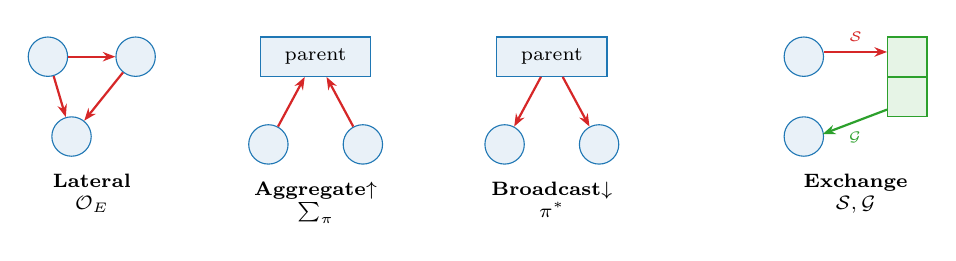
\begin{tikzpicture}[
  font=\scriptsize,
  n/.style={circle,draw=cset,fill=cset!10,minimum size=5mm,inner sep=0},
  p/.style={rectangle,draw=cset,fill=cset!10,minimum width=14mm,minimum height=5mm},
  g/.style={rectangle,draw=cfield,fill=cfield!12,minimum width=5mm,minimum height=5mm},
  a/.style={-{Stealth[length=1.6mm]},cop,thick},
]
% Lateral
\begin{scope}[local bounding box=L]
  \node[n] (a1){}; \node[n,right=6mm of a1](a2){}; \node[n,below=5mm of a1,xshift=3mm](a3){};
  \draw[a] (a1)--(a2); \draw[a] (a1)--(a3); \draw[a] (a2)--(a3);
\end{scope}
\node[below=1mm of L,align=center]{\textbf{Lateral}\\$\mathcal{O}_E$};

% Aggregate up
\begin{scope}[shift={(34mm,0)},local bounding box=A]
  \node[p] (par){parent};
  \node[n,below=6mm of par,xshift=-6mm](c1){}; \node[n,below=6mm of par,xshift=6mm](c2){};
  \draw[a] (c1)--(par); \draw[a] (c2)--(par);
\end{scope}
\node[below=1mm of A,align=center]{\textbf{Aggregate}$\uparrow$\\$\sum_\pi$};

% Broadcast down
\begin{scope}[shift={(64mm,0)},local bounding box=B]
  \node[p] (par2){parent};
  \node[n,below=6mm of par2,xshift=-6mm](d1){}; \node[n,below=6mm of par2,xshift=6mm](d2){};
  \draw[a] (par2)--(d1); \draw[a] (par2)--(d2);
\end{scope}
\node[below=1mm of B,align=center]{\textbf{Broadcast}$\downarrow$\\$\pi^*$};

% Exchange
\begin{scope}[shift={(96mm,0)},local bounding box=E]
  \node[n] (o1){}; \node[n,below=5mm of o1](o2){};
  \node[g,right=8mm of o1](g1){}; \node[g,below=0mm of g1](g2){};
  \draw[a,transform canvas={yshift=0.6mm}] (o1)-- node[above,font=\tiny]{$\mathcal{S}$}(g1);
  \draw[a,cfield,transform canvas={yshift=-0.6mm}] (g2)-- node[below,font=\tiny]{$\mathcal{G}$}(o2);
\end{scope}
\node[below=1mm of E,align=center]{\textbf{Exchange}\\$\mathcal{S},\mathcal{G}$};
\end{tikzpicture}
\caption{The four operators. \emph{Lateral} acts within a set; \emph{Aggregate}
and \emph{Broadcast} move across containment $\pi$; \emph{Exchange} scatters
($\mathcal{S}$) to and gathers ($\mathcal{G}$) from a field. P2G/G2P and the
metabolite--reaction graph are both Exchange.}
\label{fig:ops}
\end{figure}

\paragraph{Composition.} ``MPM moves the cell'' $=$ Lateral@particle then
Aggregate$\uparrow$. ``Signalling moves the cell'' $=$ Lateral@cell then
Broadcast$\downarrow$. ``Object changes field, field moves object'' $=$
$\mathcal{S}$ then $\mathcal{G}$.

\section{Dynamics: a schedule}

A model is a multi-rate composition of operators, $\;\mathcal{O}_n\circ\cdots\circ
\mathcal{O}_1$, declared as a \texttt{Schedule}. Operators are pure (return
deltas); the schedule sums per set and integrates, so rollout stays
differentiable. The LLM agentic loop searches over schedules and operator
parameterizations --- one well-defined action space instead of per-domain code.

\section{Glossary}

\begin{center}
\renewcommand{\arraystretch}{1.2}
\begin{tabular}{@{}lll l@{}}
\toprule
\textbf{Concept} & \textbf{Set/operator term} & \textbf{Symbol} & \textbf{Code} \\
\midrule
collection of like nodes & set (level)          & $S_k$                       & \texttt{Level} \\
a single node            & element              & $x\in S_k$                  & row of \texttt{Level.state} \\
learnable per-node code  & embedding            & $a_i$                       & \texttt{Level.embedding} \\
containment              & partition            & $\pi_k\!:\!S_k\!\to\!S_{k+1}$& \texttt{Level.parent} \\
within-set links         & relation             & $E\subseteq S_k\times S_k$  & \texttt{Level.edge\_index} \\
continuum quantity       & field                & $f:\Omega\to\mathbb{R}^c$   & \texttt{Field} \\
dynamics (GNN)           & operator: ODE+Laplacian & $\mathcal{O}$            & \texttt{Operator} \\
within-set op            & lateral              & $\mathcal{O}_E$             & \texttt{Lateral} \\
up op                    & reduction over fibres& $\sum_\pi$                  & \texttt{Aggregate} \\
down op                  & lift                 & $\pi^{*}$                   & \texttt{Broadcast} \\
set$\leftrightarrow$field op & transfer          & $\mathcal{S},\mathcal{G}$   & \texttt{Exchange} \\
the container            & hierarchy            & $(S_\bullet,F_\bullet,\pi_\bullet)$ & \texttt{Hierarchy} \\
the model                & composition of ops   & $\mathcal{O}_n\!\circ\!\cdots\!\circ\!\mathcal{O}_1$ & \texttt{Schedule} \\
\bottomrule
\end{tabular}
\end{center}

\end{document}
